
%%%%%%%%% MASTER -- compiles the 4 sections

\documentclass[11pt,letterpaper]{article}

\usepackage{graphicx}
\usepackage{verbatim}
\usepackage{listings}

%%%%%%%%%%%%%%%%%%%%%%%%%%%%%%%%%%%%%%%%%%%%%%%%%%%%%%%%%%%%%%%%%%%%%%%%%
\pagestyle{plain}                                                      %%
%%%%%%%%%% EXACT 1in MARGINS %%%%%%%                                   %%
\setlength{\textwidth}{6.5in}     %%                                   %%
\setlength{\oddsidemargin}{0in}   %% (It is recommended that you       %%
\setlength{\evensidemargin}{0in}  %%  not change these parameters,     %%
\setlength{\textheight}{8.5in}    %%  at the risk of having your       %%
\setlength{\topmargin}{0in}       %%  proposal dismissed on the basis  %%
\setlength{\headheight}{0in}      %%  of incorrect formatting!!!)      %%
\setlength{\headsep}{0in}         %%                                   %%
\setlength{\footskip}{.5in}       %%                                   %%
%%%%%%%%%%%%%%%%%%%%%%%%%%%%%%%%%%%%                                   %%
\newcommand{\required}[1]{\section*{\hfil #1\hfil}}                    %%
\renewcommand{\refname}{\hfil References Cited\hfil}                   %%
\bibliographystyle{plain}                                              %%
%%%%%%%%%%%%%%%%%%%%%%%%%%%%%%%%%%%%%%%%%%%%%%%%%%%%%%%%%%%%%%%%%%%%%%%%%

%PUT YOUR MACROS HERE

\date{January 21st, 2011}
\title{CS 395 Homework 1}

\author{Colby Blair}

\begin{document}
\maketitle

\begin{center}
Due January 25th, 2012 \\

Grade: \_\_\_\_\_\_\_\_\_\_\_\_\_\_\_\_\_\_\_\_
\end{center}

\thispagestyle{empty}

\pagebreak

\section*{PROBLEMS}

\subsection*{1.}
First, let run times for \textbf{insertion sort} and \textbf{merge sort} be denoted by $T_i$ and $T_m$,
 respectively. $ T_i = 8n^2 $, and $ T_m = 64 n lg(n) $, where $ lg(n) = log_2 (n) $. We can then find where
$ T_i $ beats $ T_m $ by using them in an equality:

\begin{eqnarray}
	T_i = T_m & 						& \\
	=>	& 	8 n^2 = 64 n log_2 (n)		& \\
	=>	&	8 n^2 = 64 \frac{ln(n)}{ln(2)}	& \mbox{Definition of Natural Logarithm} \\
	=>	&	n = 8 \frac{ln(n)}{ln(2)}		& \\
	=>	&	\frac{n}{ln(n)} = \frac{8}{ln(2)}	& \\
	=>	&	n = e^{ -W( - \frac{ln(n)}{8} ) } & \mbox{Product Log Function}
\end{eqnarray}

This may be a bit complicated, as I am no expert with the Product Log Function. But the values of $ n $ 
where $ T_i = T_m $ is $ \approx 43.5593 $, as seen below on a graph:

\begin{figure}[!h]
	\begin{center}
		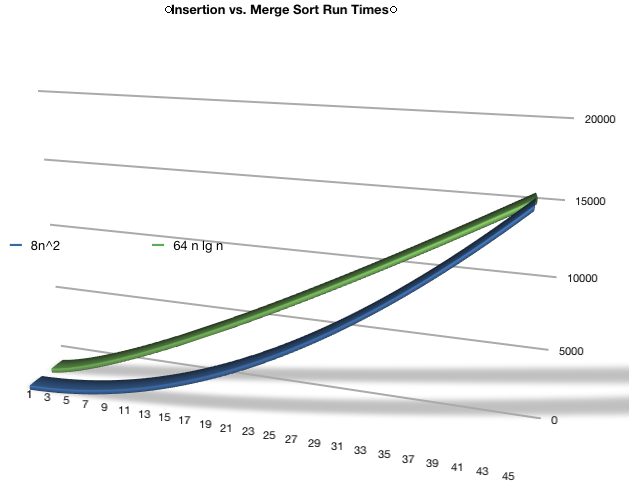
\includegraphics[width=120mm]{images/insertion_vs_merge_sort}
               	\caption{Insertion vs. Merge Sort Run Times}
                \label{insertion_vs_merge_sort}
        \end{center}
\end{figure}

As seen by the graph, \textbf{insertion sort run time beats merge sort run time for values of $ 0 < n < 43 $}.


\subsection*{2.}
The psuedocode for \textbf{linear search}:

\scriptsize
\begin{tabular}{ l l l l l l }
line&				& &			&	cost 		&	times \\
1 &	found = false		& &			&	$C_1$	&	1 \\
2 &	for i = 1 to length(A)):& & 		&	$C_2$	&	$n$ \\	
3 &	&	if A[i] $==$ some search val: 	& 	&	$C_3$	&	$ n - 1 $ \\
4 &	& &		found = true			&	$C_4$	&	$ n - 1 $ \\
\end{tabular} \\
\normalsize

We can show that the properties for a \textbf{loop invariant} hold as follows:
\begin{itemize}
	\item \textbf{Initialization:}	It can be shown that if $ A = [1] $, the array is already sorted and is trivial,
							and the loop invariant holds prior to the first interation of the loop.

	\item \textbf{Maintenance:} 	Consider the array $ A = [2,5,4] $ and $val = 4$. At line 2, $i = 1$. When
							 $i == 3$, on line 3 $ A[3] == 4 $. We then branch to line 4. 

							By Proof by Induction, since we branch into the inner 'if' statement and
							have the correct found value before leaving the 'for' loop, 
							the second invariant loop property holds.

	\item \textbf{Termination:}	Refering to the final output in the 'found' value above, the correct result
							exists on termination, and the third invariant loop property holds.
\end{itemize}


\subsection*{3.}
Considering the equation $ n^3 /  1000 - 100n^2 - 100n + 3 $, to put it into $ \Theta $-notation,
consider the leading term $ n^3 $. During the growth of $ n $, $ n ^ 3 $ grows much quicker than the rest
of the terms. So $ \Theta (n^3) $.

\pagebreak

\subsection*{4.}
Pseudo code for \textbf{selection sort} is as follows:

\scriptsize
\begin{tabular}{ l l l l l l l } 
line&	&&&						& cost	&	time \\
1&	A = [a1, a2, ... an]	&&&			& $C_1 $	&	1	\\
2&	for j = 1 to n - 1	&&&			& $C_2 $	&	$ n -1  $	\\
3&	&	min\_i = j;	&&			& $C_3 $	&	$ n - 2 $	\\
4&	&	for i = j +1 to n &&			& $C_4 $	&	$ \sum_{j=1}^{n} t_j $ \\
5&	&	&	if (A[i] < A[min\_i])	&	& $C_5 $	&	$ \sum_{j=1}^{n} (t_j - 1) $	\\
6&	&	&	&	min\_i = i;		& $C_6 $	&	$ \sum_{j=1}^{n} (t_j - 1) $	\\
7&	&	& 	i = i + 1 			&	& $C_7 $	&	$ \sum_{j=1}^{n} (t_j - 1) $	\\
8&	&	j = j + 1		&&		  	& $C_8 $	&	$ \sum_{j=1}^{n} t_j $		\\
9&	&	if min\_i != j	&&			& $C_9 $	&	$ n - 2 $	\\
10&	&	&	swap(a, j, min\_i); 	&	& $C_{10} $&	$ n - 2 $	\\
\end{tabular} \\
\normalsize

The algorithm maintains the Termination property. The algorithm needs to look and check whether to swap
many elements, and to compare them all, it only needs to run $ (n - 1) $ times.

Total time is denoted as $T(n)$:\\
$
	T(n)		= C_1 + C_2(n-1) + C_3(n-2) + C_4\sum_{j=1}^{n} (t_j - 1) + C_5\sum_{j=1}^{n} t_j
			+ C_6\sum_{j=1}^{n} t_j + C_7\sum_{j=1}^{n} t_j + C_8\sum_{j=1}^{n} (t_j - 1) + C_9(n-2) + C_{10}(n-2)
$

To find $ \Theta $ for the \textbf{worst case}, the array $ A $ is in the reverse order. Thus, $ t_j = j $ 
for $ j = 1, 2, 3... n $. Thus:

\begin{eqnarray}
	\sum_{j = 1}^{n} j = \frac{n ( n + 1 ) }{2} - 1 \\
	\sum_{j = 1}^{n} (j - 1) = \frac{n ( n + 1 ) }{2}
\end{eqnarray}

$T(n)$ can therefore be denoted as:\\
$
	T(n)		= C_1 + C_2(n-1) + C_3(n-2) + C_4( \frac{n(n+1)}{2} - 1) + C_5( \frac{n(n+1)}{2})
			C_6( \frac{n(n+1)}{2}) + C_7( \frac{n(n+1)}{2}) + C_8( \frac{n(n+1)}{2} - 1) + C_9(n-2) + C_{10}(n-2)
$ \\
$
= 	( \frac{C_4}{2} + \frac{C_5}{2} + \frac{C_6}{2} + \frac{C_7}{2} + \frac{C_8}{2} ) n^2
+	( C_2 + C_3 + \frac{C_4}{2} + \frac{C_5}{2} + \frac{C_6}{2} + \frac{C_7}{2} + \frac{C_8}{2} + C_{10}) n
+	( C_1 - C_2 - 2C_3 - C_4 - C_8 + 3C_9 - 2C_{10})
$\\
$
= an^2 + bn + c
$\\

To find $\Theta$, we take the leading term, or $an^2$. Getting rid of the constant $a$, we find that 
$\Theta$ is $\Theta(n^2)$.

To find the \textbf{best case}, find that $t_j = 1 $ for $ j = 1, 2, 3, ... n $. Therefore: \\
$
	T(n)		= C_1 + C_2(n-1) + C_3(n-2) + C_4(n - 2) + C_8(n - 2) + C_9(n-2) + C_{10}(n-2)
$ \\
$
			= ( C_2 + C_3 + C_4 + C_8 + C_9 + C_{10} ) n + ( C_1 - C_2 - 2C_3 - 2C_4 - 2C_8 - 2C_9
				-2C_{10})
$ \\
$
			= an + b
$\\

To find $\Theta$, we take the leading term, or $an$. Getting rid of the constant $a$, we find that 
$\Theta$ is $\Theta(n)$.

\end{document}
